%%%%%%%%%%%%%%%%%%%%%%%%%%%%%%%%%%%%%%%%%
% Beamer Presentation
% LaTeX Template
% Version 1.0 (10/11/12)
%
% This template has been downloaded from:
% http://www.LaTeXTemplates.com
%
% License:
% CC BY-NC-SA 3.0 (http://creativecommons.org/licenses/by-nc-sa/3.0/)
%
%%%%%%%%%%%%%%%%%%%%%%%%%%%%%%%%%%%%%%%%%

%----------------------------------------------------------------------------------------
%	PACKAGES AND THEMES
%----------------------------------------------------------------------------------------
%!TEX encoding = UTF-8 Unicode

\documentclass{beamer}
\usepackage[utf8]{inputenc}
%\usepackage[T1]{fontenc}\
\usepackage{braket}
\usepackage{verbatim}

\mode<presentation> {

\usetheme{Warsaw}

}

\usepackage{graphicx} % Allows including images
\usepackage{booktabs} % Allows the use of \toprule, \midrule and \bottomrule in tables

%----------------------------------------------------------------------------------------
%	TITLE PAGE
%----------------------------------------------------------------------------------------

\title[Quantum metrology]{Quantum metrology} % The short title appears at the bottom of every slide, the full title is only on the title page

\author[Federico Belliardo]
{
Federico Belliardo\\
\vspace{10pt}
\small Relatore: Vittorio Giovannetti
} 

\institute[SNS] % Your institution as it will appear on the bottom of every slide, may be shorthand to save space
{
Scuola Normale Superiore \\ % Your institution for the title page
\medskip
}
\date{24 Aprile 2018} % Date, can be changed to a custom date

\begin{document}

\begin{frame}
\titlepage % Print the title page as the first slide
\end{frame}

%\begin{frame}
%\frametitle{Overview} % Table of contents slide, comment this block out to remove it
%\tableofcontents % Throughout your presentation, if you choose to use \section{} and \subsection{} commands, these will automatically be printed on this slide as an overview of your presentation
%\end{frame}

%----------------------------------------------------------------------------------------
%	PRESENTATION SLIDES
%----------------------------------------------------------------------------------------

\begin{frame}{Sommario}
\begin{itemize}
\item Stima dei parametri classica e quantistica 
\vspace{10pt}
\item Teoria della misura quantistica
\vspace{10pt}
\item Ottimizzazioni (stimatore, misura, probe)
\vspace{10pt}
\item Stimatore adattivo
\vspace{10pt}
\item Heisenberg scaling
\end{itemize}
\end{frame}

\begin{frame}{Stima dei parametri}
\begin{center}

Sistema caratterizzato da un parametro $\theta_0$.

\begin{figure}[!htb]
\centering
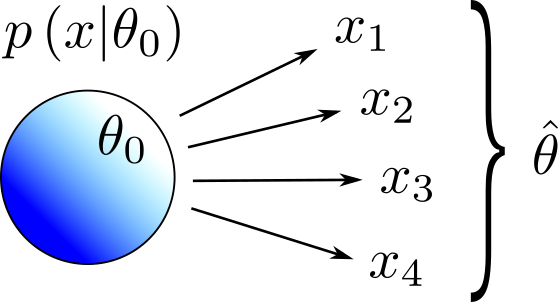
\includegraphics[scale=.50]{parameterEstimation.png}
\end{figure}

\begin{itemize}
\item Misura: interrogazione del sistema produce $x$ con $p(x | \theta_0)$.
%La meccanica classica in alcuni casi fornisce delle probabilità (meccaica statistica)... qualche volta è interna alla fisica
\item Data processing: costruzione dello stimatore $\hat{\theta} \left( x_1, x_2, ..., x_n \right)$
%Si suppone che lo stimatore abbia qualcosa a che fare con il valore di \theta_0.
\end{itemize}

Esiste un limite alla precisione di $\hat{\theta}$?
\end{center}
\end{frame}


%------------------------------------------------

\begin{frame}
\frametitle{Limite di Cramér-Rao e informazione di Fisher}

\begin{block}{Limite di Cramér-Rao}
Sia $\hat{\theta} \left( \vec{x} \right) $ stimatore di $\theta$ con $\vec{x}$ vettore delle misure. Esiste un lower bound sulla sua varianza:

\[
Var \left( \hat{\theta} \right) \geq \frac{1}{N I \left( \theta \right)} 
\]


con $N$ numero di misure, dove $I \left( \theta \right)$ è detta \textbf{informazione di Fisher} ed è definita come:

\[
I \left( \theta \right) = \mathbb{E} \left[ \left( \frac{\partial \log p \left(x, \theta \right) }{\partial \theta} \right) ^ 2 \right] = - \mathbb{E} \left[ \frac{\partial^2 \log p \left(x, \theta \right)}{\partial \theta^2} \right]
\]

%per misure indipendenti $I \left( \theta \right) = N I_1(\theta)$.

\end{block}
%Essa è additiva per misure indipendenti.
\begin{center}

%\[
%\frac{\partial \mathcal{L}}{\partial \theta} \left( \hat{\theta} \right)  = 
%\frac{\partial \log p \left( \vec{x}, \theta \right)}{\partial \theta} \left( %\hat{\theta} \right) = 0
%\]

%Dire che asintoticamene efficiente vuol proprio dire che satura cramer rao
Il maximum likelyhood estimator è asintoticamente efficiente, cioè:
$ Var \left( \hat{\theta}_{ML} \right) \rightarrow \frac{1}{N I \left( \theta \right)}$ per $N \rightarrow \infty$.

\end{center}
\end{frame}

%------------------------------------------------

\begin{frame}{Stima dei parametri quantistica}
\begin{center}

In MQ il parametro $\theta$ che caratterizza un sistema è codificato nello stato $\rho_{\theta}$.

Esempi: $\rho_{\beta} = \frac{1}{Z} e^{-\beta H}$ (temperatura), $\ket{\psi}_{\phi} = \frac{\ket{0} + e^{i \phi} \ket{1}}{\sqrt{2}}$ (fase interferometrica), ...

\begin{figure}[!htb]
\centering
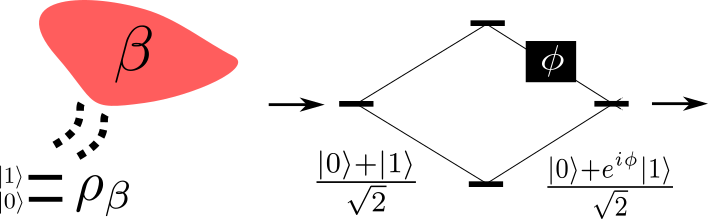
\includegraphics[scale=.50]{example.png}
\end{figure}

\end{center}
\end{frame}

\begin{frame}{Stima dei parametri quantistica}
\begin{center}
Il processo di misura è costituito dall'interazione di una \textit{probe} $\rho_0$ con il sistema caratterizzato da $\theta$. L'interazione è rappresentata da un generico canale quantistico (CPT). 

\begin{figure}[!htb]
\centering
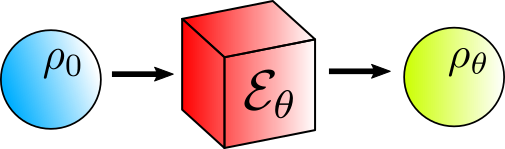
\includegraphics[scale=.50]{channel.png}
\end{figure}
\[ \rho_0 \rightarrow  \mathcal{E}_{\theta}(\rho) = \rho_{\theta} \]

Bisogna formulare il problema di stima in termini della teoria della misura quantistica!
Le misure sono distruttive: è necessario utilizzare molti $\rho_{\theta}$.

\end{center}
\end{frame}

\begin{frame}{Teoria della misura quantistica}
\begin{center}
POVM: \textit{Positive Operator Valued Measure}

\begin{figure}[!htb]
\centering
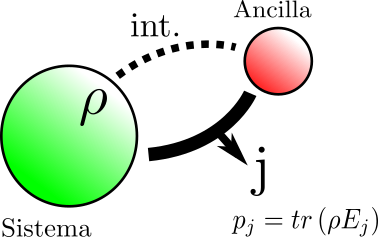
\includegraphics[scale=.50]{POVM.png}
\end{figure}

\begin{itemize}
\item Interazione con ancilla
\item Misure proiettive sul sistema \textit{joint}
\end{itemize}

$\rho$ è la matrice densità ridotta del sistema

$0 \leq E_j \leq \mathbb{I} \quad p_j = tr \left( \rho E_j \right) \quad \sum_{j} E_{j} = \mathbb{I}$

La distribuzione di probabilità $p \left( j, \theta \right)$ dipende dalla misura! Si può ottimizzare la POVM per massimizzare l'informazione estratta.

\end{center}
\end{frame}

%\begin{center}
%\textbf{E' possibile sfruttare la meccanica quantistica per aumentare la precisione delle misure?}
%\end{center}



%Mediante un canale quantistico: 

%\[
%\rho \rightarrow \mathcal{E}_{\theta} \left( \rho \right) = \rho_{\theta}
%\]

\begin{comment}
\begin{frame}
\frametitle{Quantum parameter estimation}

\begin{center}

Si possono estrarre informazioni da $\rho_{\theta}$ attraverso una POVM (): $\{E_x\}$ con $0 \leq E_x \geq \mathbb{I}$ e  $\sum_{j} E_{j} = \mathbb{I}$, la probabilità di ottenere $x$ è: $p_{E} \left( x, \theta \right) = tr \left( \rho_{\theta} E_x \right)$.


\begin{block}{}
\begin{center}
Si può ottimizzare la POVM da eseguire in modo da massimizzare l'informazione estratta da $\rho_{\theta}$.
\end{center}
\end{block}
%Segue l'analisi dati per ricavare lo stimatore $\hat{\theta}$.
\end{center}

\end{frame}

\end{comment}


%------------------------------------------------

\begin{frame}
\frametitle{Quantum Fisher Information}
\begin{center}

%Consideriamo il caso in cui $\rho_{\theta} = e^{- i \theta A} \rho e^{- i \theta A}$. 

\begin{block}{Quantum Fisher Information}
Si definisce $QFI \left( \theta \right)$ la massima informazione di Fisher che si può estrarre variando la POVM applicata su $\rho_{\theta}$:
\[
QFI \left( \theta \right) = \max_{POVM} I \left( \theta \right)
\]
\end{block}

%La $QFI \left( \theta \right)$ è la minima funzione convessa di $\rho$ che si riduce a $4 (\Delta A)^2_{\psi}$ sugli stati puri.

%Dire due parole sulla fidelity: essa codifica quanto due stati sono vicini (è una distanza tra stati) 
La QFI è esprimibile come derivata della distanza di Bures tra stati:
\[
D_{B} (\rho_1, \rho_2) = \sqrt{2} \left[ 1 - \Big| \text{Tr} \sqrt{\sqrt{\rho_1} \rho_2 \sqrt{\rho_1}} \Big| \right]^{\frac{1}{2}}
\]
\[
QFI \left( \theta \right) = 4 \lim_{\delta \rightarrow 0} \frac{D^{2}_{B} \left( \rho_{\theta + \delta}, \rho_{\theta} \right)}{\delta^2}
\]
%dove $F (\rho_1, \rho_2) = \Big| \text{Tr} \sqrt{\sqrt{\rho_1} \rho_2 \sqrt{\rho_1}} \Big| ^ 2  $ è la \textit{fidelity}.
\end{center}
\end{frame}

\begin{frame}{Quantum Fisher Information}
\begin{center}

$S = \left\{ \rho_{\theta}, \theta \in \Theta \right\} $ è una traiettoria 1D nello spazio degli stati quantistici.

\begin{figure}[!htb]
\centering
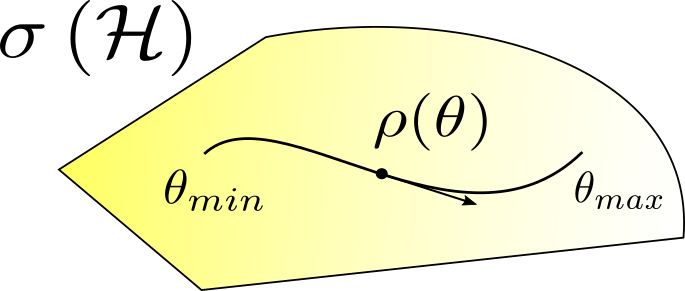
\includegraphics[scale=0.7]{traiettoria.png}
\end{figure}


La $QFI \left( \theta \right)$ codifica la velocità con cui gli stati quantistici lungo la linea diventano \textbf{distinguibili} l'uno dall'altro.

%proprietà della QFI, symmetric logharitmic derivative. Usarla come parametro per quantificare entanglement (k saparable)...

\end{center}
\end{frame}

\begin{frame}{Proprietà della QFI}
\begin{center}

Consideriamo il caso in cui $\rho_{\theta} = e^{- i \theta H} \rho e^{+ i \theta H}$ (interferometro di Ramsey, Mach-Zehnder, ...). Per uno stato puro $\ket{\psi_k}$:

\[ QFI \left( \theta \right) = 4 \left( \Delta H \right)^2_{\psi_k} \]

\textbf{Relazione di indeterminazione energia-tempo} 

\[ Var \left( \hat{\theta} \right) = \left( \Delta \theta \right)^2_{\psi_k} \geq \frac{1}{ 4 \left( \Delta H \right)^2_{\psi_k}} \rightarrow  \Delta \theta \Delta H \geq \frac{1}{2} \]
\end{center}
\end{frame}

\begin{frame}{Proprietà della QFI}
\begin{center}

%Essa si riduce a $4 \left( \Delta H \right)^{2}_{\psi_k}$ per gli stati puri.
La POVM ottimale ($I = QFI$) per estrarre informazione da $\rho_{\theta}$ è costituita dai proiettori sugli autospazi dell'operatore $L_{\theta}$ chiamato \textit{ symmetric logarithmic derivative} che soddisfa a:
\[ \frac{\partial \rho_{\theta}}{\partial \theta} = \frac{1}{2} \left( \rho_{\theta} L_{\theta} + L_{\theta} \rho_{\theta} \right) \]

In generale la POVM ottimale dipende da $\theta$. Ma il valore vero $\theta_0$ non è noto a priori! E' necessario utilizzare una \textbf{strategia adattiva}.

\end{center}
\end{frame}

\begin{frame}{Ottimizzazioni}
\begin{center}
Riassunto sulle possibilità di ottimizzazione:
\vspace{5pt}
\begin{itemize}
\item Stimatore $\hat{\theta}$
\vspace{5pt}
\item POVM (Nuova!) - problema della dipendenza da $\theta_0$ della misura ottimale
\vspace{5pt}
\item Probe $\rho_0$ (Nuova!)
\vspace{5pt}
\end{itemize}

La convessità della $QFI \left( \theta \right)$ assicura che l'informazione è massima per gli stati $\rho_0$ puri.

%La $QFI(\theta)$ per uno stato $\rho$ è minore della massima $QFI(\theta)$ degli stati puri in un ensamble rappresentato da $\rho$. Possiamo dunque limitarci a usare stati puri come probes.
\end{center}
\end{frame}

\begin{frame}{Strategie con entanglement}
\begin{center}


%Si ha una serie di  \textit{probes} (qubit) inizializzate in uno stato $\rho_0$. Esse interagiscono con il sistema di cui si vuole misurare il parametro $\theta$: $\rho_0 \rightarrow  \mathcal{E}_{\theta}(\rho) = \rho_{\theta}$

E' possibile far interagire $m$ probes tra loro prima dell'applicazione di $\mathcal{E}_{\theta}$ creando dunque uno stato \textbf{entangled}:

%Cosa succede se si fanno interagire le probes? Prima e dopo?...

\begin{figure}[!htb]
\centering
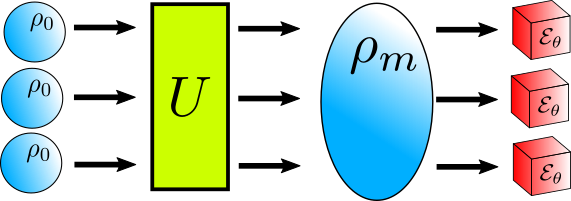
\includegraphics[scale=.50]{entanglement.png}
\end{figure}
\[
\underbrace{\rho_0 \otimes \rho_0 \otimes ... \otimes \rho_0}_{m} \rightarrow \rho_{m}
\]

Può l'entanglement migliorare la precisione delle misure?

\end{center}
\end{frame}

\begin{frame}{QFI per stati entangled}
\begin{center}


Identificata la $QFI \left( \theta \right)$ come figura di merito per la precisione di una stimatore possiamo chiederci quanto vale per uno stato $\rho_N$ costituito da $N$ probe.
Si osserva che:
\[
QFI_{\rho^{\otimes N}} \left( \theta \right) = N QFI_{\rho}  \left( \theta \right)
\] 
\[\quad H = \sum_{i = 1}^{N} h_i\]
\[QFI_{\rho^{\otimes N}} \left( \theta \right) = 4 \left( \Delta H \right)^2 = 4 \sum_{i=1}^{N}  \left( \Delta h_i \right)^2  = N QFI_{\rho}  \left( \theta \right)\]

cioè $QFI$ scala come il numero $N$ di probe per stati separabili.

\end{center}
\end{frame}

\begin{frame}{QFI per stati entangled}
\begin{center}

Per un generico stato $\rho_N$ di $N$ probe abbiamo:
\[QFI_{\rho_N} \left( \theta \right) = 4 \left( \Delta H \right)^2 \leq N^2\]

dunque: \[QFI_{\rho_N} \leq N^2\]

\begin{block}{\textbf{Heisenberg scaling?}}
\[
Var \left( \hat{\theta} \right) \propto \frac{1}{N^2} \quad (N \rightarrow \infty)
\]
\end{block}

\end{center}
\end{frame}

\begin{comment}
\begin{frame}{QFI per stati entangled}
\begin{center}

\begin{block}{Stati $k$-producibili}
\begin{center}
Uno stato $\ket{\psi}$ è detto k-producibile se è scrivibile come $\ket{\psi} = \ket{\psi_1} \otimes \ket{\psi_2} \otimes ... \otimes \ket{\psi}$. Dove $\ket{\psi_m}$ sono stati di al più $k$ particelle.
\end{center}
\end{block}

Per uno stato $k$-producibile l'informazione di Fisher è limitata da:
\[ QFI \left( \theta \right) \leq s k^2 + \left( N - sk \right) ^2 \quad s = \lfloor \frac{N}{k} \rfloor \]

Per la quantum metrology è necessario \textbf{entanglement multipartito}.

\end{center}
\end{frame}
\end{comment}


\begin{frame}{QFI per stati entangled}

\begin{center}

%TODO: Aggiungere anche per ognuno di essi quanto vale la Qfisher
Vediamo alcuni esempi di stati utili:
\vspace{10pt}
%GHZ NON è  SPIN SQUEEZED, dipende quale definizione si da.
\begin{itemize}
\item $\ket{\psi}_{NOON} = \frac{\ket{N, 0} + \ket{0, N}}{\sqrt{2}} \rightarrow \frac{\ket{N, 0} + e^{i N \theta} \ket{0, N}}{\sqrt{2}}$ $\theta$ misurabile $mod \, \frac{2 \pi}{N}$, sensing, stati tipici di interferometri, $QFI \left( \theta \right) = N^2$

\vspace{10pt}
\item $\ket{\psi}_{GHZ} = \frac{\ket{0}^{\otimes N} + \ket{1}^{\otimes N}}{\sqrt{2}}$ (come sopra)
%\vspace{10pt}
%\item $\ket{\psi}_{Dicke} = {{N}\choose{m}}^{\frac{1}{2}} \sum_{k} {\mathcal{P}_k \ket{1}%^{\otimes m} \otimes \ket{0}^{\otimes N-m}}$ 
\vspace{10pt}
%(spin squeezing)
%In egnerale si parla di spin squeezed state come stati di particelle a spin 1/2 utili per la metrologia
%Esempi di stati entanglati in sistemi di spin 1/2. Sono esempi di stati spin squeezed?
%\item $\vec{J} = \sum_{i} \vec{\sigma}_{i} \quad \xi^2 = \frac{N ( \Delta J_{n_3})^2}{\langle J_{n_1} \rangle ^2 + \langle J_{n_2} \rangle ^2} < 1$ (Spin squeezed states) 
%\item Wiseman-Berry state TODO
%\item $\ket{\psi} = \int d \mathbf{\alpha} f( \mathbf{\alpha} ) \ket{\mathbf{\alpha}}$ (Entangled coherent states, numero di particelle non fissato)
\end{itemize}

Gli stati entangled evolvono $N$ volte più velocemente degli stati separabili (in termini di distinguibilità).
\end{center}
\end{frame}


%Cosa succede se uso l'entanglement (in un interferometro)? Mostro heisenberg scaling negli interferometri (stile advances in quantum metrology). Non mi convince che gli stati ghz siano davvero utili per stimare la fase.

%Nel caso della stima di temperatura si possono avere più sistemi non commutanti che sono alla stessa temperatura (sistema entangled attraverso l'ambiente anche se sono  non interagenti.). Però comunque ci riduciamo sempre a diagonalizzare una sola stessa hamiltoniana. Inoltre non corrisponde al mio setting.

%$Var(\hat{\theta}) \geq \frac{1}{M \sqrt{\nu}}$

%(Si ottiene qualcosa di simile anche ne caso termometrico?)

%Osservazione: se tutte le misure fanno parte di un unico blocco entangled allora $Var (\hat{\theta}) \geq \frac{1}{M} = \frac{1}{N}$. Lo stimatore di massima likelyhood (per la misura ottimale) raggiunge asintoticamente la quantum Fisher Information.

%applicazioni: biologia (campioni fotosensibili), onde gravitazionali (lavorare al limite di danneggiamento dello specchio),... Devo ancora dire delle cose su l fatto che gli stati GHZ permettono di fare sensing e che devo usare stratege con un numero crescente di blocchi entangled
%Posso anche non aggiornare tutte le volte e fujiwara funziona.
%Dovrei dire qualcosa sul fatto che si possa raggiungere l'Heisemberg scaln anche senza la fase di adattamento.

\begin{frame}{Stimatore adattivo}
\begin{center}

Dimentichiamo l'entanglement per ora.

Per raggiungere il quantum Cramér-Rao bound  si utilizza uno stimatore MLE addattivo:

\begin{figure}[!htb]
\centering
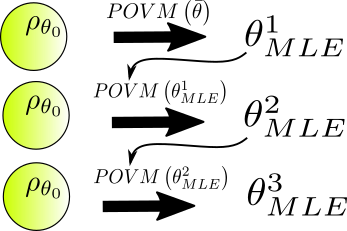
\includegraphics[scale=.50]{adattivo.png}
\end{figure}


La bontà di uno stimatore è caratterizzata da:

\begin{itemize}
\item Consistenza: $\theta^{n}_{MLE} \rightarrow \theta_0$ per $n \rightarrow +\infty$
\item Efficienza: $Var \left( \theta^{n}_{MLE} \right) \rightarrow \frac{1}{n QFI(\theta_0)}$, la definizione classica prevede $I(\theta_0)$
\end{itemize}
\end{center}
\end{frame}

\begin{frame}{Consistenza ed efficienza}
\begin{center}
Consistenza forte ed efficienza dello stimatore di massima likelyhood adattivo.

\begin{itemize}
\item $x \in X$ spazio risultati delle misure (discreto)
\item $\theta \in \Theta$ spazio dei parametri (compatto)
\item $e \in E$ spazio degli esperimenti (compatto)

\end{itemize}

Ipotesi: conosciamo il miglior esperimento $\hat{e}(\theta)$ associato ad ogni valore $\theta$ (si ottiene diagonalizzando la SLD).

$f(x_n, \theta, e_n)$ è la probabilità di misurare il valore $x_n$ eseguendo la POVM $e_n$ sullo stato $\rho_{\theta}$.
\[ \hat{\theta}_{MLE} = arg \max_{\theta} \prod_{i = 1}^{n} f \left( x_i, \theta, e_i \right) \]
\end{center}
\end{frame}

\begin{frame}{Consistenza ed efficienza}
\begin{center}
\begin{block}{Teorema (Fujiwara 2006)} 
\begin{center}
Supponiamo che il valore vero del parametro sia $\theta_0$ e che la misura $e_n$ sia scelta sulla base del risultato delle misure precedenti: $e_{n} = \hat{e} \left( \hat{\theta}_{n-1} (x_1, x_2, ..., x_{n-1}) \right)$
allora
\[
\sqrt{n} \left( \hat{\theta}_n - \theta_0 \right) \rightarrow N \left( 0, QFI(\theta)^{-1} \right)
\]
\end{center}
\end{block}
\end{center}
Ipotesi:
\begin{itemize}
\item $f(x, \theta, e) > 0$ per ogni $(x, \theta, e)$, continua in $(x, \theta, e)$.
\item $\mu \left( {x | f(x, \theta, e) \neq f(x, \theta', e)} \right) > 0$ per ogni $\theta \neq \theta'$, $e \in E$.
\item  $f(x, \theta, e)$ è $C^3$ in $\theta$.
\end{itemize}

\begin{center}
La tesi rimane vera anche se non si aggiorna subito la POVM da eseguire.
\end{center}

\end{frame}


\begin{frame}
\begin{center}
Passaggi fondamentali della dimostrazione:
\begin{itemize}
\item Si dimostra che $P_{\theta_0} \left[ |\hat{\theta}_n - \theta_0|  \geq a \right] \leq e^{- b n}$ con $b > 0$. $b$ dipende dalla misura, dallo stato iniziale $\rho_0$ e da $a$.
%COME SI SCRIVEREBBE IN ITALIANO INFINITELY OFTEN
\item $P_{\theta_0} \left[ |\hat{\theta}_n - \theta_0|  \geq a \; i. o. \right] = 0$. L'evento $|\hat{\theta}_n - \theta_0|  \geq a$ accade un numero finito di volte. Questo prova la consistenza forte dello stimatore adattivo.
\item Definiamo $\mathcal{L}(\theta | x, e) = \log f(x, \theta, e)$ e $\mathcal{L}_n (\theta) = \sum_{i=1}^{n} \mathcal{L}( \theta | x_i, e_i)$. Sviluppiamo a primo ordine: $\mathcal{L}^{'}_n(\theta) = \mathcal{L}^{'}_n \left( \theta_0 \right) + \mathcal{L}^{''}_n \left( \theta_0 \right) \left( \theta - \theta_0 \right) + \frac{1}{2} \mathcal{L}^{'''}_n (\theta^*) (\theta-\theta_0)^2$. $\mathcal{L}^{'}_n(\hat{\theta}_n) = 0$ per definizione di MLE, dunque:
\[
\sqrt{n} \left( \hat{\theta}_n - \theta_0 \right) = \frac{ \frac{\mathcal{L}^{'}_n \left( \theta_0 \right) }{\sqrt{n}}}{
- \frac{\mathcal{L}^{''}_n (\theta_0)}{n} - \frac{\mathcal{L}^{'''}_n \left( \theta^{*} \right) }{2 n} \left( \hat{\theta}_n - \theta_0 \right)}
\]

\end{itemize}

\end{center}
\end{frame}

\begin{frame}
\begin{center}
\begin{itemize}

%Attenzione in realtà dove dico in probabilità si tratta di convergenze quasi certe. Però per dimostrare il teorema (l'fficienza) mi basta la convergenza in probabilità. Anche il pezzo a denominatore dove c'è la differenza dello stimatore con \theta_0 tensde fortemente a 0 in effetti.
\item $\frac{\mathcal{L}^{'''}_n \left( \theta^{*} \right) }{2 n} \leq M $ in probabilità: vi è un numero finito di $n$ per cui la disuguaglianza non è verificata. $-\frac{\mathcal{L}^{'''}_n}{2 n} \left( \hat{\theta}_n - \theta_0 \right) \rightarrow 0$.

%: $sup_{X \times B_{\delta}(\theta_0) \times E} \Big| \mathcal{L}^{'''} \left( \theta | x, e \right) \Big| \leq M \rightarrow \Big| \frac{\mathcal{L}^{'''}_n (\theta*)}{n} \Big| \leq M \quad P_{\theta_0} q.c.$ TODO

%DIRE CHE LA FI RAGGIUNGE IL VALORE OTTIMALE.
\item $\frac{\mathcal{L}^{''}_n (\theta_0)}{n} \rightarrow -QFI \left( \theta_0 \right)$ in probabilità: l'informazione osservata media tende alla $QFI \left( \theta_0 \right)$.
\item $ \frac{\mathcal{L}^{'}_n \left( \theta_0 \right)}{\sqrt{n}} \rightarrow N(0, QFI \left( \theta_0 \right))$ in distribuzione.
\end{itemize}

\begin{block}{Teorema}
\begin{center}
$\lbrace X_n \rbrace \rightarrow  X$ in distribuzione e $\lbrace Y_n \rbrace \rightarrow c$ in probabilità allora $\frac{X_n }{Y_n} \rightarrow \frac{X}{c}$ in distribuzione.
\end{center}
\end{block}
\[
\sqrt{n} \left( \hat{\theta}_n - \theta_0 \right)  \rightarrow \frac{ N \left( 0, QFI \left( \theta_0 \right) \right)}{QFI \left( \theta_0 \right) } = N \left( 0, QFI \left( \theta_0 \right) ^ {-1} \right)
\]

\end{center}
\end{frame}

\begin{frame}{Varianza asintotica}
\begin{center}
Cosa possiamo dire sulla raggiungibilità dell'Heisenberg scaling?

\begin{block}{}
\[
Var \left( \hat{\theta} \right) \propto \frac{1}{N^2} \quad (N \rightarrow \infty)
\]
\end{block}

Lo stimatore adattivo raggiungere asintoticamente la varianza:
\[
Var \left( \hat{\theta}_n - \theta_0 \right) \rightarrow \frac{1}{n QFI (\theta_0)}
\]
Se eseguiamo la stima su $n$ blocchi entangled di $M$ probe il cui stato è stato scelto in maniera ottimale si ha $QFI \left( \theta_0 \right) = M^2$, $N_{tot} = M n$. La varianza asintotica diventa: \[ Var \left( \hat{\theta}_n - \theta_0 \right) \rightarrow \frac{n}{N_{tot}^2} \]

\end{center}
\end{frame}

\begin{frame}{Heisenberg scaling}
\begin{center}

Non è chiaro se a $N_{tot}$ fissato esiste una nozione di scaling: 

%Dipendenza di N^{0}_{tot} da \epsilon?
dato $\epsilon  > 0$, per $N_{tot} > N^{0}_{tot}$ fissato $\exists \, n_0 \; | \; n > n_0$ si ha: \[ \Big| Var \left( \hat{\theta}_n - \theta_0 \right) \frac{N_{tot}^2}{n}  - 1 \Big| < \epsilon \]

In generale il valore $n_0$ da cui comincia a valere il risultato asintotico può dipendere dal valore $N_{tot}$ così che la varianza per $n_0$ misure sia:
\[
Var \left( \hat{\theta}_n - \theta_0 \right) \sim \frac{n_0 (N_{tot})}{N^{2}_{tot}}
\]

%Se $n_0$ è indipendente da $N_{tot}$:


\textbf{Heisenberg scaling?}


\end{center}
\end{frame}

\begin{frame}{Heisenberg scaling}
\begin{center}

%Notiamo che deve essere scelto uno stato che permetta di distinguere tutte le fasi $\theta \in [0, 2 \pi)$ per poter applicare il teorema di sopra, questo avrà sicuramente una $QFI(\theta)$ minore di $M^2$. 

%$ \ket{\psi} = \ket{GHZ}_{M-1} \otimes \left( \frac{\ket{0}_{M} + \ket{1}_{M}}{\sqrt{2}} \right) $

%In generale per gli stati 2-producibili vale: $ QFI(\theta) \leq (M-1)^2 + 1 = M^2 - 2M + 2$

%TODO: Lo stato scritto sopra satura la varianza massima per i 2-producibili?

%Questo cambia la varianza asintotica che diventa:

%\[
%Var \left( \hat{\theta} - \theta_0 \right) \rightarrow \frac{\sqrt{n}}{N_{tot} \sqrt{1 - %\frac{2}{M} + \frac{2}{M^2}}}
%\]

Nello schema di Fujiwara non si possono utilizzare subito blocchi entangled, per via della limitata regione di sensibilità ($\theta \, mod \, \frac{2 \pi}{M}$).

\begin{figure}[!htb]
\centering
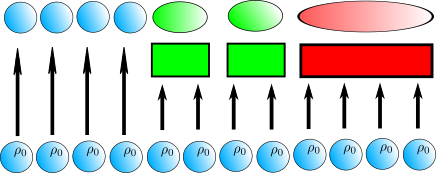
\includegraphics[scale=.70]{strategia.png}
\end{figure}

E' necessaria una strategia in cui si varia la dimensione del blocco di qubit entangled (aumentandola esponenzialmente), oltre che il numero di ripetizioni. Non contemplata da Fujiwara perché la $QFI$ non ha limite in questi schemi (cresce con $M$).

%Per $M = 1$ questa strategia è legata all'algoritmo di \textit{quantum phase estimation}.


\end{center}
\end{frame}

\begin{frame}{Heisenberg scaling}
\begin{center}

\textbf{Rimane un problema aperto la raggiungibilità dell'Heisenberg scaling in qualche schema!}

\end{center}
\end{frame}

%\begin{frame}

%Per concludere la diostrazione di Fujiwara funziona anche se non si aggiorna subtito la misura ottimale.
%Non è in effetti possibile formulare il problema in termini di variaziona dello stimatore di massima likelyhood perché tutte le volte che si aumenta il grado di entanglement del blocco si cambia il dominio della distribuzione di probabilità così che se si vuole massimizzare la likelyhood $\mathbb{L}$ sul dominio non è possibile farlo su $[0, 2\pi]$ ma se lo si fa sul dominio degli ultimi blocchi allora è necessario quantificare con quale precisione di può affermare che $\theta$ si trova nell'intervallo scelto e ricadiamo nel problema originale. La precisione della misura è limitata dai primi blocchi con poco entanglement. Se queste misure sono scadenti non importa quanto precise saranno quelle successive con molto entanglement. Avrò comunque una probabilità consistente di sbagliare la localizzazione di $\theta$ di molto e dunque una grande varianza.


%Se si massimizza su $[0, 2\pi]$ si ottiene una distribuzione oscillante (nel caso di due stage per esempio) e la risoluzione dello stimatore dipende dalla precisione del primo stage.

%Test delle ipotesi continuo?  E' un procedimento bayesiano sostanzialmente equivalente alla stima bayesiana dei parametri dove ogni volta la prior viene aggiornata con al posterior precendete. La prior iniziale è ovviamente uniforme.
%Neanche questo metodo sembra dare particolari vantaggi.

%\end{frame}

%------------------------------------------------


\begin{frame}
\frametitle{Bibliografia} 
\footnotesize{
\begin{thebibliography}{99} % Beamer does not support BibTeX so references must be inserted manually as below

%\bibitem https://arxiv.org/pdf/1109.3128.pdf
%\bibitem Quantum metrology and its application in biology
%\bibitem https://arxiv.org/pdf/1405.4878.pdf

\bibitem -Géza Tóth and Iagoba Apellaniz, Quantum metrology from a quantum information science perspective, 2014 \emph{J. Phys. A: Math. Theor.} 47 424006


\bibitem -Akio Fujiwara, Strong consistency and asymptotic efficiency for
adaptive quantum estimation problems, 2006 \emph{J. Phys. A: Math. Gen.} 39 12489

\end{thebibliography}
}
\vspace{30pt}
\Huge{\centerline{Grazie per l'attenzione!}}

\end{frame}

%----------------------------------------------------------------------------------------

\end{document} 